\documentclass[a4paper]{article}
\usepackage[english]{babel}
\usepackage{multicol}
\usepackage{amsmath}
\usepackage{amsfonts}
\usepackage{amssymb}
\usepackage{graphicx}
\usepackage[font=scriptsize]{caption}
\usepackage{parskip}
\usepackage[a4paper, margin= 1in ,total={6in, 8in}]{geometry}
\usepackage{titling}
\usepackage{subcaption}
\usepackage{float}
\usepackage{placeins}

\parskip = 6pt plus 2pt minus 2pt
\setlength{\droptitle}{-2cm}

\title{HW2- Computer Simulation II}
\author{Schewtschik, Guilherme  (3748052)}
\date{\today}

\begin{document}

\maketitle

\section{}
For this task the spins are plotted in a 2d grid, where the color of the cell represents the value of the spin.

\begin{figure*}[ht]
    \centering
    \begin{subfigure}{0.45\textwidth}
        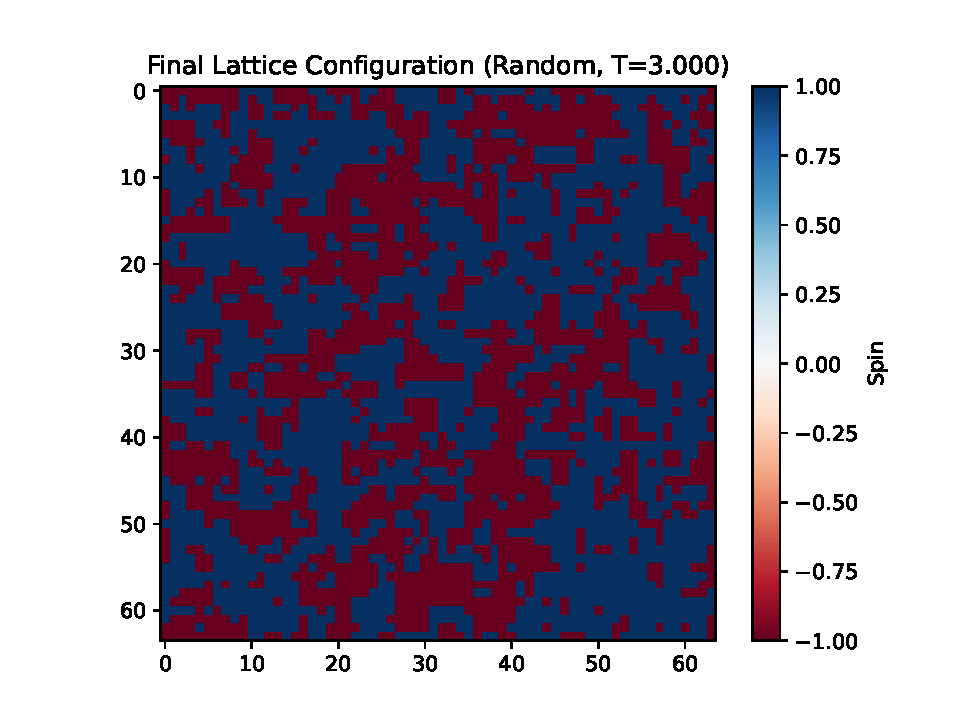
\includegraphics[width=\textwidth]{plots/Random_0.pdf}
        
    \end{subfigure}

     \begin{subfigure}{0.45\textwidth}
        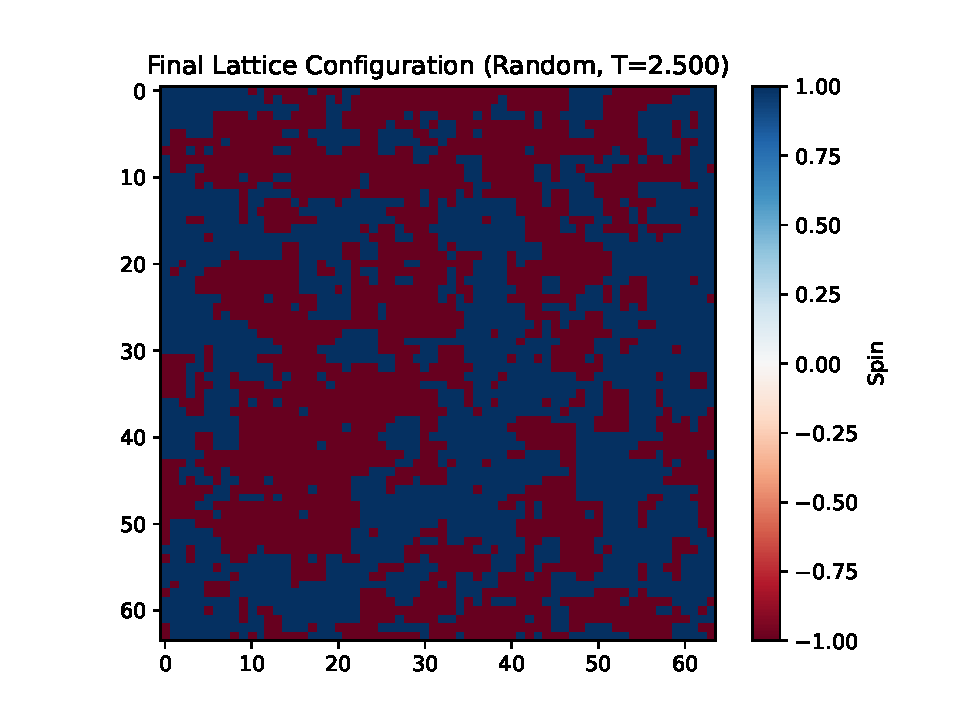
\includegraphics[width=\textwidth]{plots/Random_1.pdf}
        
    \end{subfigure}
    \hfill
    \begin{subfigure}{0.45\textwidth}
        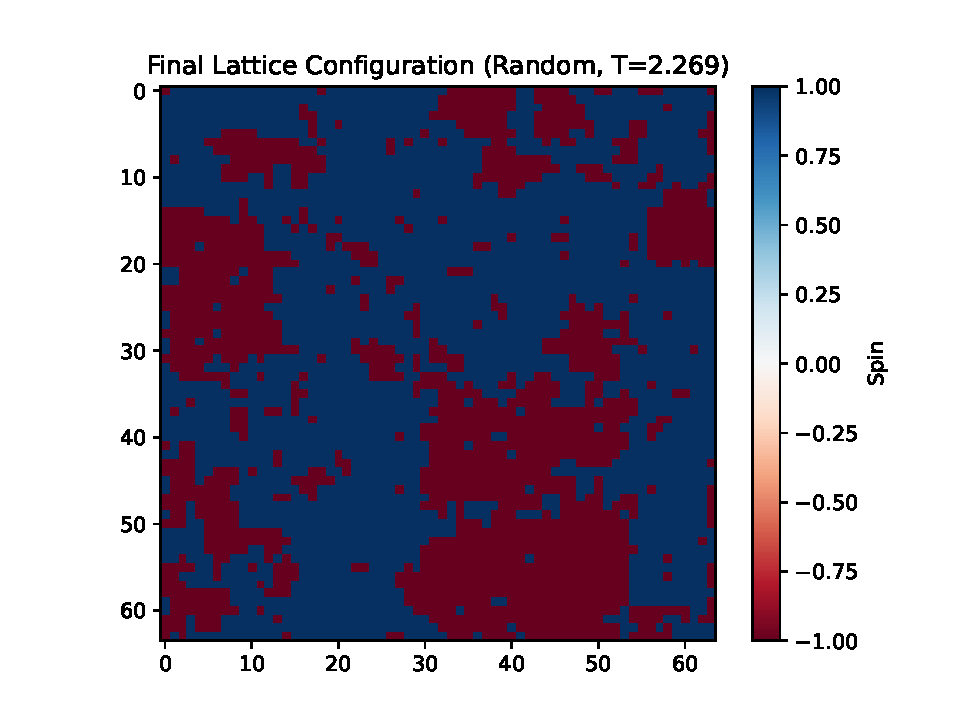
\includegraphics[width=\textwidth]{plots/Random_2.pdf}
        
    \end{subfigure}

     \begin{subfigure}{0.45\textwidth}
        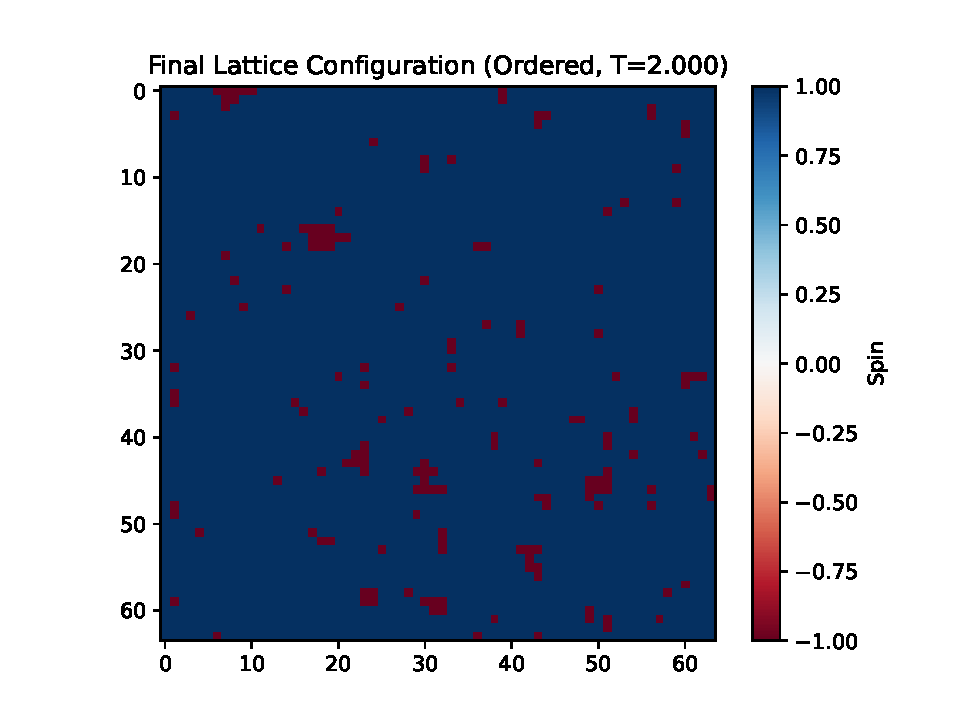
\includegraphics[width=\textwidth]{plots/Ordered_3.pdf}
        
    \end{subfigure}
    \hfill
    \begin{subfigure}{0.45\textwidth}
        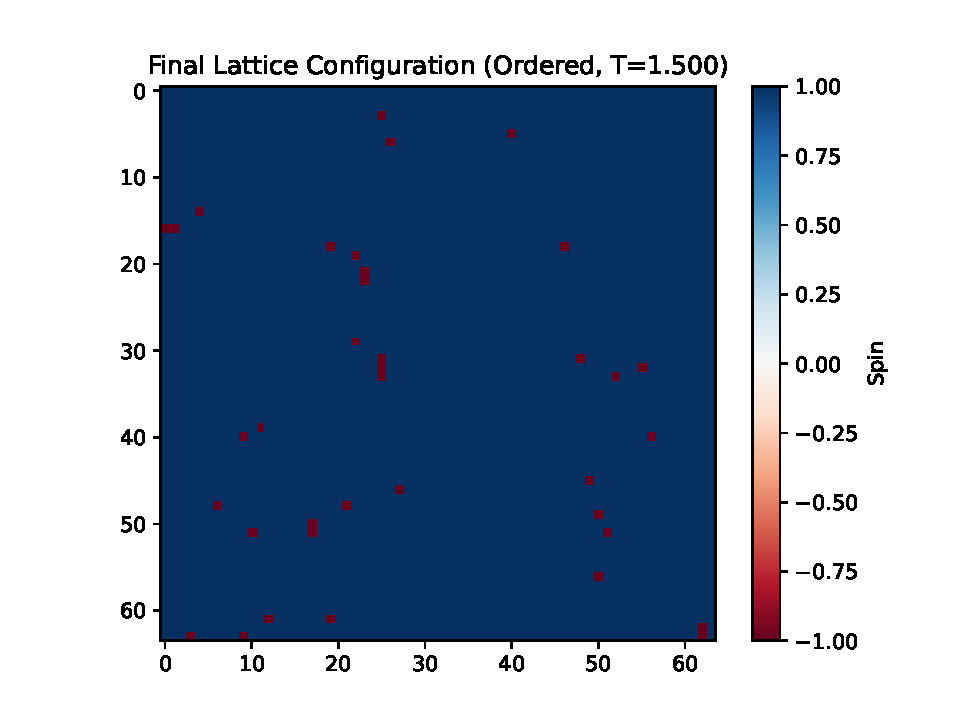
\includegraphics[width=\textwidth]{plots/Ordered_4.pdf}
        
    \end{subfigure}

\end{figure*}

We can see the alignment of the spin 
directions with the lowering of temperature which is 
the expected result. The first three plots show a global net 
zero magnetization with only local alignment, while the last two
show a global net magnetization with all spins aligned in the same direction.

\newpage

\section{}
Utilizing the same Wolff algorithm implemented in the previous homework, we arrive at the 
following graphs for the Energy per spin $E$, and the specific heat $C$ around the critical temperature $T_c$.

\begin{figure}[ht]
\centering

\begin{subfigure}{0.48\textwidth}
    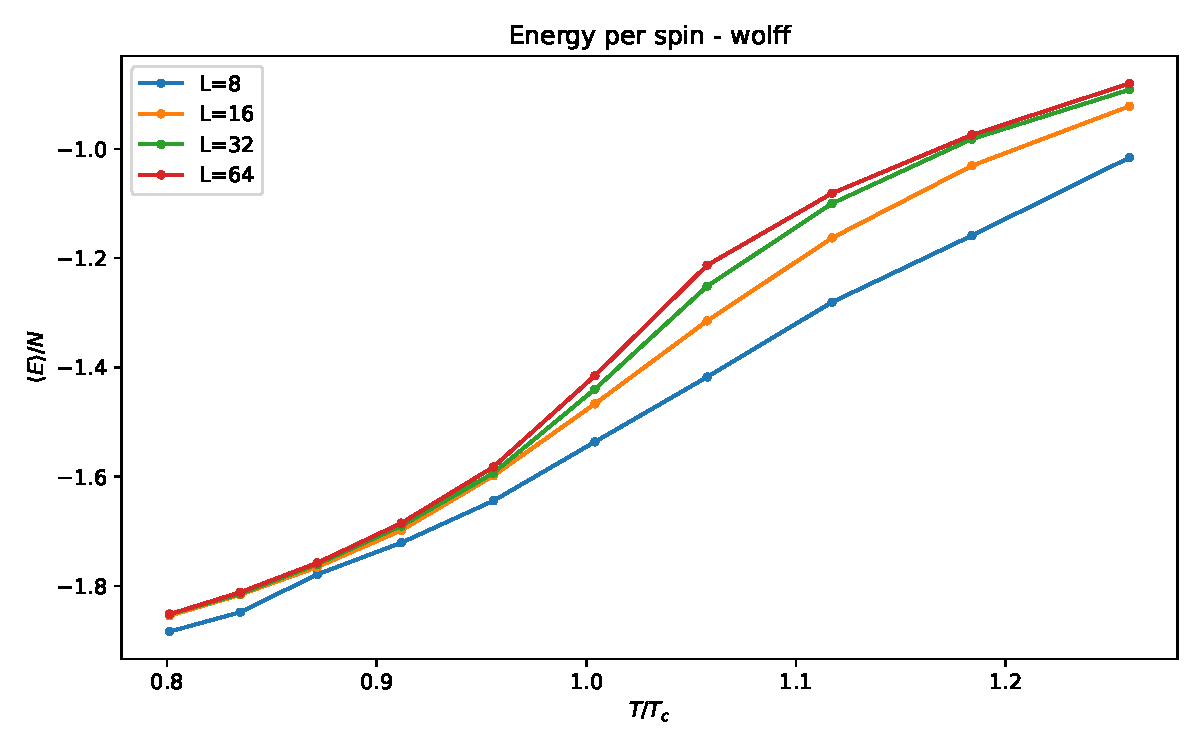
\includegraphics[width=\linewidth]{plots/E_per_spin_T.pdf}
\end{subfigure}
\hfill
\begin{subfigure}{0.48\textwidth}
    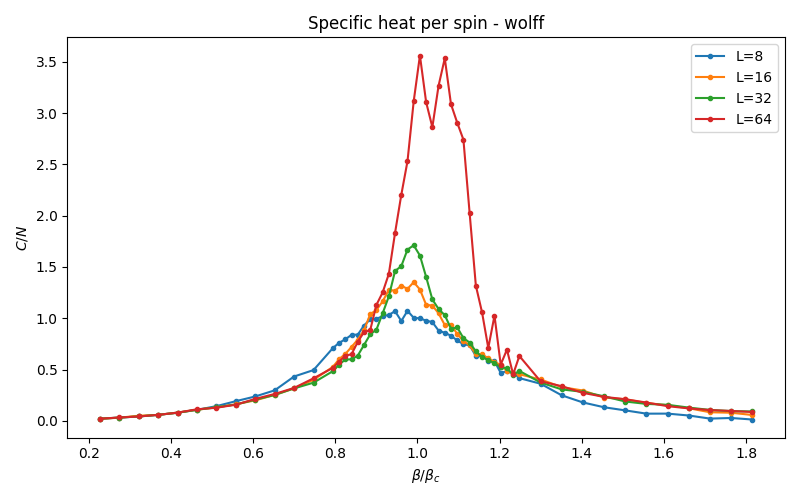
\includegraphics[width=\linewidth]{plots/Specific_heat_res.png}
\end{subfigure}

\end{figure}

We can also plot the values obtained from the module homepage and get:

\begin{figure}[ht]
\centering

\begin{subfigure}{0.48\textwidth}
    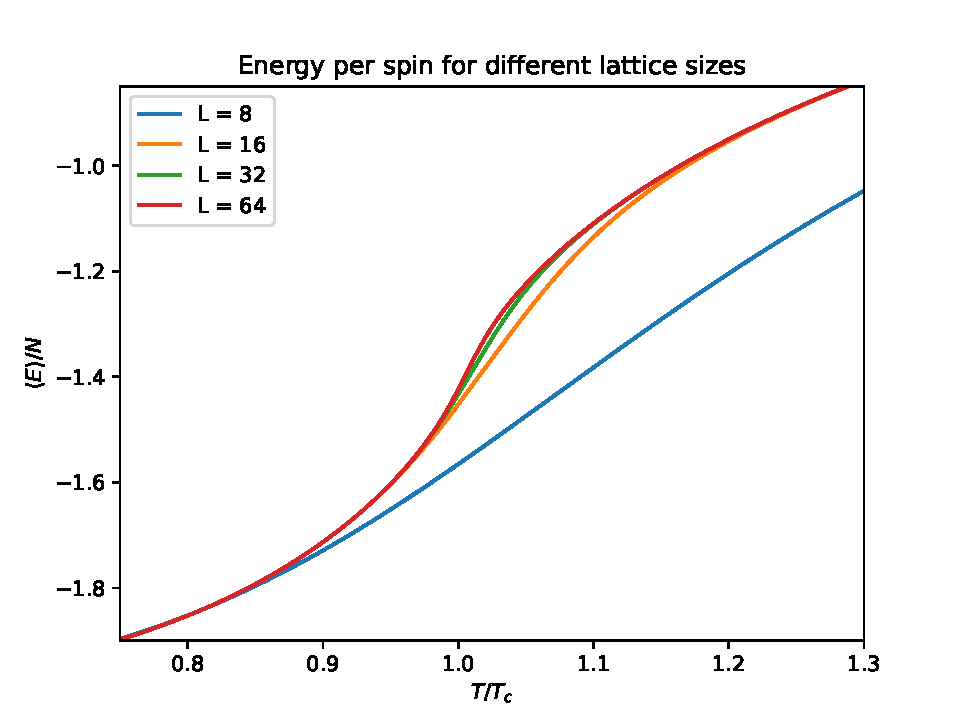
\includegraphics[width=\linewidth]{plots/E_per_spin_T_prof.pdf}
\end{subfigure}
\hfill
\begin{subfigure}{0.48\textwidth}
    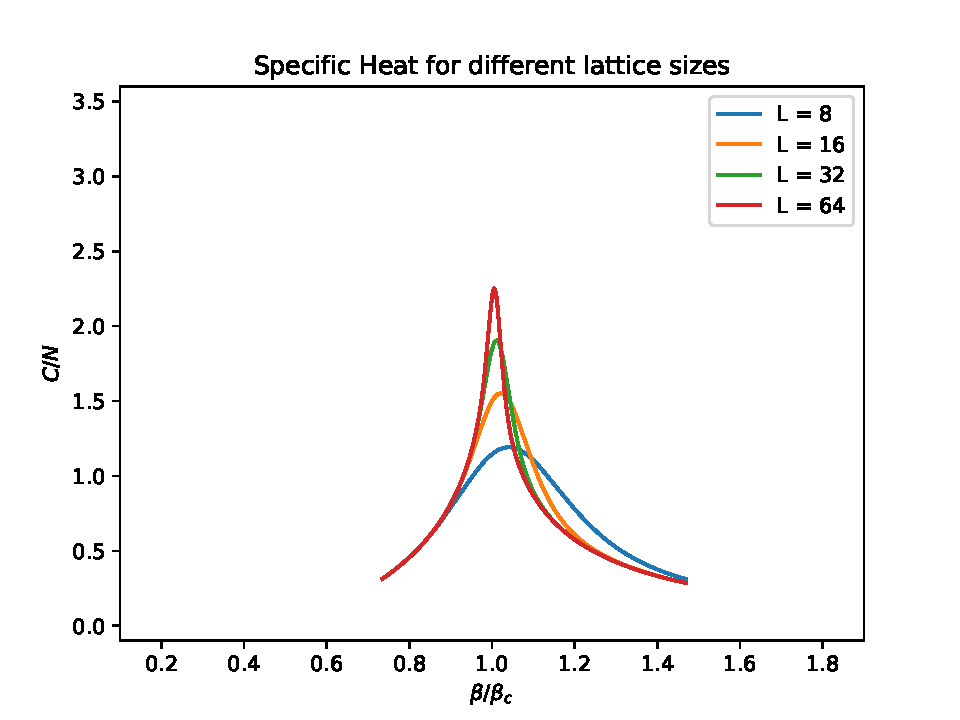
\includegraphics[width=\linewidth]{plots/Specific_heat_prof.pdf}
\end{subfigure}

\end{figure}

We can clearly see that the values obtained from our simulation are in good agreement with the values 
obtained from the module homepage only presenting some minor deviations, specially for the heat capacity, 
where the peak value for the $L=64$ grid surpasses the expected result by quite a lot.
We can also see that the specific heat has a peak around the critical temperature $T_c$, 
which is a characteristic feature of phase transitions.


We estimate the scaling of the autocorrelation time near the critical temperature using the ansatz
\[
\tau(L) \sim L^z.
\]
A linear fit in log--log space is used to extract the dynamical exponent \(z\).

For the Wolff (cluster) algorithm, we obtain:

\begin{itemize}
    \item Energy:
    \[
    z_E = -0.70 \pm 0.56, \qquad R^2 = 0.43
    \]

    \item Magnetization:
    \[
    z_M = -0.99 \pm 1.01, \qquad R^2 = 0.32
    \]
\end{itemize}


\end{document}
